\chapter{Conceptos previos}


\section{Machine Learning}

Se entiende como el campo de las ciencias de computación que en vez de enfocarse en el diseño de algoritmos explícitos, optan por el estudio de técnicas de aprendizaje. Este enfoque tiene un gran éxito en tareas computacionales donde no es factible diseñar un algoritmo de forma explícita. \cite{Programming_Massively} \\
En vez de averiguar las distintas reglas a seguir para llegar a una solución, esta alternativa permite simplemente suministrar ejemplos de lo que debería pasar en distintas situaciones, y dejar que la máquina aprenda y extraiga ella misma sus propias conclusiones. De esta forma, el procedimiento en aprendizaje supervisado consiste en 'entrenar' con una muestra de N ejemplos, extraer información de ellos, y posteriormente poder evaluar de forma 'correcta' (bajo un margen de error controlado) otra muestra de M ejemplos, siendo M \textgreater N. \cite{Learning_From_Data} \\
Este enfoque ha contribuido en el avance de áreas como reconocimiento de voz, visión por ordenador, procesamiento de lenguaje natural, etc.


\section{Deep Learning}

\section{Tipos de aprendizaje}

\subsection{Aprendizaje Supervisado}

% \cite{Learning_From_Data} página 24

Es el que se empleará en este proyecto. 
Se caracteriza por la presencia de una etiqueta 'correcta' $y_i$ asociada a cada dato de entrada $x_i$. Posteriormente, la red empleará ambos valores para, a partir de $x_i$, tratar de deducir $y_i$. \cite{Learning_From_Data} \\
Aunque se tratará de impedirlo, siempre hay ruido en los datos empleados, implicando que algunas etiquetas de Y=$\{y_1, y_2, ..., y_N\}$ pueden ser erróneas. \\

\subsection{Aprendizaje No Supervisado}

En este tipo de aprendizaje, los datos no contienen ninguna información respecto a lo que debe predecir la red. De esta forma, el conjunto de datos D se compone exclusivamente de valores X=$\{x_1, x_2, ..., x_N\}$. \cite{Learning_From_Data}

\subsection{Aprendizaje Por Refuerzo}

En este caso tampoco existe un $y_i$ 'correcto' asociado a cada $x_i$. En su lugar, se asocia a cada $x_i$ una etiqueta con un valor posible de $y_i$, además de una medida que indica como de bueno es el mismo. \cite{Learning_From_Data}


\section{Tipos de problemas en machine learning}

\subsection{Clasificación}
\subsection{Regresión}

\section{Componentes necesarios para el aprendizaje supervisado}

Datos de entrada X y de salida Y que el modelo empleará para aprender y tomar decisiones. Ambos se unen para formar un dataset de entradas-salidas D=\{($x_1, y_1$), ($x_2, y_2$), ..., ($x_N, y_N$)\}. Para que el aprendizaje sea posible, debe existir una función F: X $\rightarrow$ Y tal que $y_i$ = F($x_i$) para i$\in$\{1...N\}. De esta forma, en función del dataset D, el modelo tratará de encontrar una función G que aproxime F para dicho conjunto. Además, se suelen aplicar técnicas que permitan una mejor generalización del modelo, expandiendo las capacidades del mismo y permitiendo que su conocimiento pueda ser útil incluso fuera de la muestra de datos inicial. \cite{Learning_From_Data}

\section{Entrenamiento}

\section{División de datos en entrenamiento y test}

Para permitir la generalización del modelo, D se suele dividir en 2 subconjuntos, (entrenamiento y test) de forma que se pueda estimar si realmente 'aprende' o solo memoriza.\\
Una vez realizada la división, se entrena el modelo con los datos del conjunto de entrenamiento. Una vez finalizado, se accede al conjunto test y se visualiza el rendimiento del modelo sobre el mismo. Como los datos de test no se emplearon en todo el proceso de entrenamiento, aportan una estimación sobre la generalización del modelo fuera de la muestra con la que se entrenó. 


\section{Redes Neuronales Totalmente Conectadas}

\subsection{Neurona}

\begin{figure}[H]
	\centering
	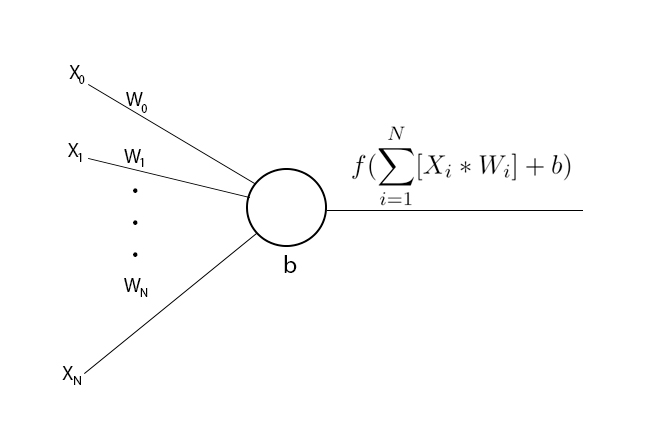
\includegraphics[scale=0.35]{imagenes/neurona.jpg}  
	\caption{Imagen de una neurona}
	\label{fig:neurona}
\end{figure}

Una neurona se compone de una serie de datos de entrada X=\{$x_1$, $x_2$, ..., $x_N$\} tal que cada $x_i$$\in${X} se encuentra asociado a un peso $w_i\in{W}$. \\
La neurona los emplea para realizar una suma ponderada y posteriormente añadir un bias b, además de aplicar una función de activación f sobre el resultado obtenido. 

\subsection{Estructura por capas}

\begin{figure}[H]
	\centering
	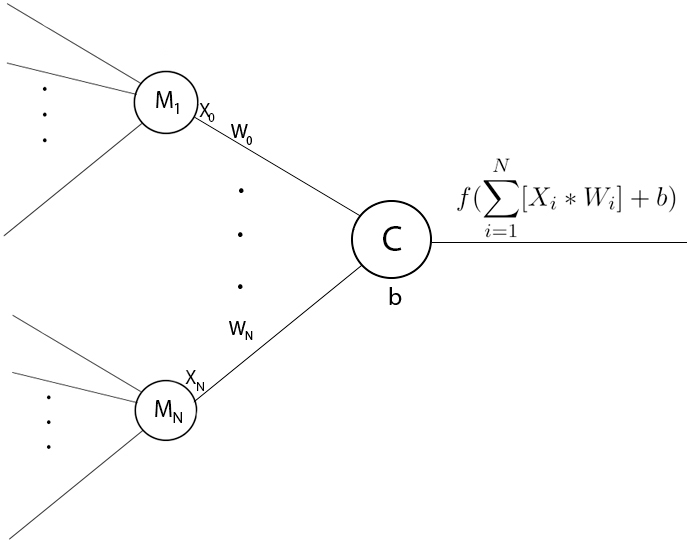
\includegraphics[scale=0.35]{imagenes/capa_neuronas.jpg}  
	\caption{Imagen de una capa de neuronas}
	\label{fig:capa_neuronas}
\end{figure}

Las neuronas se suelen agrupas por capas, de tal forma que la salida de una compone la entrada de la siguiente, formando así modelos más sofisticados.

\subsection{Funciones de activación}

\subsubsection{ReLU}

\begin{gather}
	ReLU(x) = max(0, x)
\end{gather}

\begin{figure}[H]
	\centering
	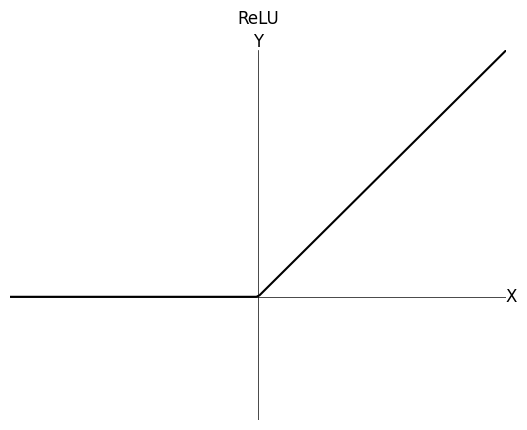
\includegraphics[scale=0.45]{imagenes/ReLU.jpg}  
	\caption{Imagen de la función de activación ReLU}
	\label{fig:ReLU}
\end{figure}

A cambio de un bajo coste computacional, aporta no linealidad a la neurona, permitiendo a esta aprender funciones de mayor complejidad. \\
Como su gradiente es 0 o 1, evita una reducción excesiva del mismo para valores positivos, mitigando así el problema del desvanecimiento del gradiente, caracterizado por la presencia de gradientes muy pequeños en backpropagation y provocar un aprendizaje lento. \cite{ReLU}

\subsubsection{Sigmoide}

\begin{gather}
	sigmoide(x) = \frac{1}{1+e^{-x}}
\end{gather}

\begin{figure}[H]
	\centering
	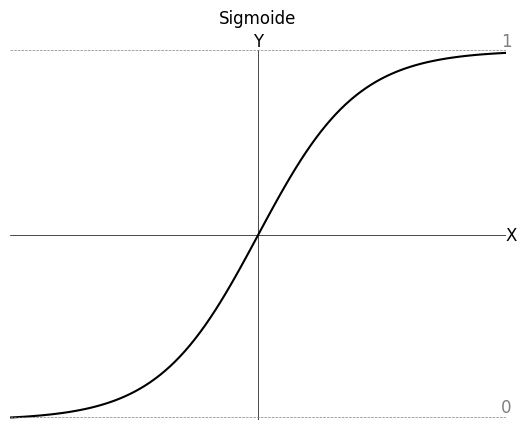
\includegraphics[scale=0.45]{imagenes/sigmoide.jpg}  
	\caption{Imagen de la función de activación Sigmoide}
	\label{fig:Sigmoide}
\end{figure}

Se trata de una función interesante en el ámbito de la clasificación binaria, pues se caracteriza por transformar un valor de entrada en una salida comprendida en el rango [0-1]. \\
Aunque sea monótona creciente y diferenciable en todos los puntos, tiende a saturarse con valores extremos (positivos o negativos). Por tanto, su aplicación dependerá del caso concreto a tratar. \cite{Sigmoide}

\subsubsection{SoftMax}

\begin{figure}[H]
	\centering
	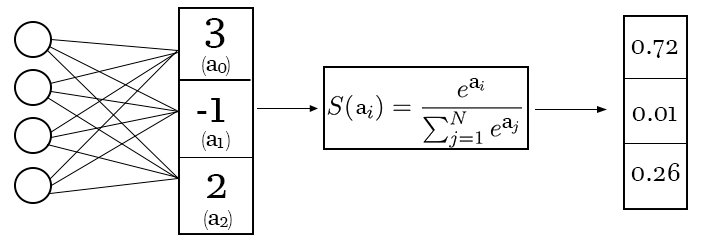
\includegraphics[scale=0.35]{imagenes/softmax.jpg}  
	\caption{Imagen de la función de activación SoftMax}
	\label{fig:SoftMax}
\end{figure}

Para n entradas, produce n salidas con valores en el rango [0-1] que mantienen la proporción de entrada y cuya suma es 1. Por tanto, se pueden interpretar como la probabilidad de pertenencia a cada clase, siendo especialmente útil en clasificación multiclase. \cite{SoftMax_MLM} \\
\subsection{One-hot encoding}

\subsection{Función de error o pérdida}
% https://medium.com/mlearning-ai/understanding-loss-functions-for-classification-81c19ee72c2a

Como solo tenemos dos clases y estamos en clasificación binaria, usaremos Sigmoid Cross Entropy Loss.

\begin{gather}
   H(x) = - \frac{1}{N} \sum_{i=1}^{N}  [y_i * log( \hat{y}_i) + (1-y_i)*log(1-\hat{y_i})]
   \label{loss_func}
\end{gather}

y = etiqueta real \\
$\hat{y}$ = predicción 

\subsection{ForwardPropagation}
\subsection{Descenso del gradiente}
Es un método de optimización que busca el mínimo local en una función diferenciable.

\subsection{BackPropagation}
Regla de la cadena

\section{Redes Neuronales Convolucionales}

\subsection{Tipos de capas}

\subsection{Estructura por capas}

\subsection{ForwardPropagation}
